\documentclass[11pt,a4paper,]{article}
\usepackage{lmodern}

\usepackage{amssymb,amsmath}
\usepackage{ifxetex,ifluatex}
\usepackage{fixltx2e} % provides \textsubscript
\ifnum 0\ifxetex 1\fi\ifluatex 1\fi=0 % if pdftex
  \usepackage[T1]{fontenc}
  \usepackage[utf8]{inputenc}
\else % if luatex or xelatex
  \usepackage{unicode-math}
  \defaultfontfeatures{Ligatures=TeX,Scale=MatchLowercase}
\fi
% use upquote if available, for straight quotes in verbatim environments
\IfFileExists{upquote.sty}{\usepackage{upquote}}{}
% use microtype if available
\IfFileExists{microtype.sty}{%
\usepackage[]{microtype}
\UseMicrotypeSet[protrusion]{basicmath} % disable protrusion for tt fonts
}{}
\PassOptionsToPackage{hyphens}{url} % url is loaded by hyperref
\usepackage[unicode=true]{hyperref}
\hypersetup{
            pdftitle={Gender stereotypes in Israel},
            pdfborder={0 0 0},
            breaklinks=true}
\urlstyle{same}  % don't use monospace font for urls
\usepackage{geometry}
\geometry{a4paper, centering, text={16cm,24cm}}
\usepackage[style=authoryear-comp,]{biblatex}
\addbibresource{references.bib}
\usepackage{longtable,booktabs}
% Fix footnotes in tables (requires footnote package)
\IfFileExists{footnote.sty}{\usepackage{footnote}\makesavenoteenv{long table}}{}
\usepackage{graphicx,grffile}
\makeatletter
\def\maxwidth{\ifdim\Gin@nat@width>\linewidth\linewidth\else\Gin@nat@width\fi}
\def\maxheight{\ifdim\Gin@nat@height>\textheight\textheight\else\Gin@nat@height\fi}
\makeatother
% Scale images if necessary, so that they will not overflow the page
% margins by default, and it is still possible to overwrite the defaults
% using explicit options in \includegraphics[width, height, ...]{}
\setkeys{Gin}{width=\maxwidth,height=\maxheight,keepaspectratio}
\IfFileExists{parskip.sty}{%
\usepackage{parskip}
}{% else
\setlength{\parindent}{0pt}
\setlength{\parskip}{6pt plus 2pt minus 1pt}
}
\setlength{\emergencystretch}{3em}  % prevent overfull lines
\providecommand{\tightlist}{%
  \setlength{\itemsep}{0pt}\setlength{\parskip}{0pt}}
\setcounter{secnumdepth}{5}

% set default figure placement to htbp
\makeatletter
\def\fps@figure{htbp}
\makeatother


\title{Gender stereotypes in Israel}

%% MONASH STUFF

%% CAPTIONS
\RequirePackage{caption}
\DeclareCaptionStyle{italic}[justification=centering]
 {labelfont={bf},textfont={it},labelsep=colon}
\captionsetup[figure]{style=italic,format=hang,singlelinecheck=true}
\captionsetup[table]{style=italic,format=hang,singlelinecheck=true}


%% FONT
\RequirePackage{bera}
\RequirePackage[charter,expert,sfscaled]{mathdesign}
\RequirePackage{fontawesome}

%% HEADERS AND FOOTERS
\RequirePackage{fancyhdr}
\pagestyle{fancy}
\rfoot{\Large\sffamily\raisebox{-0.1cm}{\textbf{\thepage}}}
\makeatletter
\lhead{\textsf{\expandafter{\@title}}}
\makeatother
\rhead{}
\cfoot{}
\setlength{\headheight}{15pt}
\renewcommand{\headrulewidth}{0.4pt}
\renewcommand{\footrulewidth}{0.4pt}
\fancypagestyle{plain}{%
\fancyhf{} % clear all header and footer fields
\fancyfoot[C]{\sffamily\thepage} % except the center
\renewcommand{\headrulewidth}{0pt}
\renewcommand{\footrulewidth}{0pt}}

%% MATHS
\RequirePackage{bm,amsmath}
\allowdisplaybreaks

%% GRAPHICS
\RequirePackage{graphicx}
\setcounter{topnumber}{2}
\setcounter{bottomnumber}{2}
\setcounter{totalnumber}{4}
\renewcommand{\topfraction}{0.85}
\renewcommand{\bottomfraction}{0.85}
\renewcommand{\textfraction}{0.15}
\renewcommand{\floatpagefraction}{0.8}


%\RequirePackage[section]{placeins}

%% SECTION TITLES


%% SECTION TITLES (NEW: Changing sections and subsections color)
\RequirePackage[compact,sf,bf]{titlesec}
\titleformat*{\section}{\Large\sf\bfseries\color[rgb]{0.8, 0.7, 0.1 }}
\titleformat*{\subsection}{\large\sf\bfseries\color[rgb]{0.8, 0.7, 0.1 }}
\titleformat*{\subsubsection}{\sf\bfseries\color[rgb]{0.8, 0.7, 0.1 }}
\titlespacing{\section}{0pt}{2ex}{.5ex}
\titlespacing{\subsection}{0pt}{1.5ex}{0ex}
\titlespacing{\subsubsection}{0pt}{.5ex}{0ex}


%% TITLE PAGE
\def\Date{\number\day}
\def\Month{\ifcase\month\or
 January\or February\or March\or April\or May\or June\or
 July\or August\or September\or October\or November\or December\fi}
\def\Year{\number\year}

%% LINE AND PAGE BREAKING
\sloppy
\clubpenalty = 10000
\widowpenalty = 10000
\brokenpenalty = 10000
\RequirePackage{microtype}

%% PARAGRAPH BREAKS
\setlength{\parskip}{1.4ex}
\setlength{\parindent}{0em}

%% HYPERLINKS
\RequirePackage{xcolor} % Needed for links
\definecolor{darkblue}{rgb}{0,0,.6}
\RequirePackage{url}

\makeatletter
\@ifpackageloaded{hyperref}{}{\RequirePackage{hyperref}}
\makeatother
\hypersetup{
     citecolor=0 0 0,
     breaklinks=true,
     bookmarksopen=true,
     bookmarksnumbered=true,
     linkcolor=darkblue,
     urlcolor=blue,
     citecolor=darkblue,
     colorlinks=true}

\usepackage[showonlyrefs]{mathtools}
\usepackage[no-weekday]{eukdate}

%% BIBLIOGRAPHY

\makeatletter
\@ifpackageloaded{biblatex}{}{\usepackage[style=authoryear-comp, backend=biber, natbib=true]{biblatex}}
\makeatother
\ExecuteBibliographyOptions{bibencoding=utf8,minnames=1,maxnames=3, maxbibnames=99,dashed=false,terseinits=true,giveninits=true,uniquename=false,uniquelist=false,doi=false, isbn=false,url=true,sortcites=false}

\DeclareFieldFormat{url}{\texttt{\url{#1}}}
\DeclareFieldFormat[article]{pages}{#1}
\DeclareFieldFormat[inproceedings]{pages}{\lowercase{pp.}#1}
\DeclareFieldFormat[incollection]{pages}{\lowercase{pp.}#1}
\DeclareFieldFormat[article]{volume}{\mkbibbold{#1}}
\DeclareFieldFormat[article]{number}{\mkbibparens{#1}}
\DeclareFieldFormat[article]{title}{\MakeCapital{#1}}
\DeclareFieldFormat[article]{url}{}
%\DeclareFieldFormat[book]{url}{}
%\DeclareFieldFormat[inbook]{url}{}
%\DeclareFieldFormat[incollection]{url}{}
%\DeclareFieldFormat[inproceedings]{url}{}
\DeclareFieldFormat[inproceedings]{title}{#1}
\DeclareFieldFormat{shorthandwidth}{#1}
%\DeclareFieldFormat{extrayear}{}
% No dot before number of articles
\usepackage{xpatch}
\xpatchbibmacro{volume+number+eid}{\setunit*{\adddot}}{}{}{}
% Remove In: for an article.
\renewbibmacro{in:}{%
  \ifentrytype{article}{}{%
  \printtext{\bibstring{in}\intitlepunct}}}

\AtEveryBibitem{\clearfield{month}}
\AtEveryCitekey{\clearfield{month}}

\makeatletter
\DeclareDelimFormat[cbx@textcite]{nameyeardelim}{\addspace}
\makeatother

\author{\sf\Large\textbf{ James Louis Nguyen}\\ {\sf\large B.Com\\[0.5cm]} \sf\Large\textbf{ Samuel Lyubic}\\ {\sf\large B.Com\\[0.5cm]} \sf\Large\textbf{ Siddhant Tirodkar}\\ {\sf\large B.Com\\[0.5cm]} \sf\Large\textbf{ Jimmy Effendy}\\ {\sf\large B.Com\\[0.5cm]}}

\date{\sf\Date~\Month~\Year}
\makeatletter
\lfoot{\sf Nguyen, Lyubic, Tirodkar, Effendy: \@date}
\makeatother


%%%% PAGE STYLE FOR FRONT PAGE OF REPORTS

\makeatletter
\def\organization#1{\gdef\@organization{#1}}
\def\telephone#1{\gdef\@telephone{#1}}
\def\email#1{\gdef\@email{#1}}
\makeatother
  \organization{Monash University}

  \def\name{Econometrics and Business Statistics}

  \telephone{(03) 9905 2478}

  \email{questions@company.com}                 %NEW: New email addresss

\def\webaddress{\url{http://company.com/stats/consulting/}} %NEW: URl
\def\abn{12 377 614 630}                                    % NEW: ABN
\def\logo{\includegraphics[width=6cm]{logo}}  %NEW: Changing logo
\def\extraspace{\vspace*{1.6cm}}
\makeatletter
\def\contactdetails{\faicon{phone} & \@telephone \\
                    \faicon{envelope} & \@email}
\makeatother

%%%% FRONT PAGE OF REPORTS

\def\reporttype{Report for}

\long\def\front#1#2#3{
\newpage
\begin{singlespacing}
\thispagestyle{empty}
\vspace*{-1.4cm}
\hspace*{-1.4cm}
\hbox to 16cm{
  \hbox to 6.5cm{\vbox to 14cm{\vbox to 25cm{
    \logo
    \vfill
    \parbox{6.3cm}{\raggedright
      \sf\color[rgb]{0.8, 0.7, 0.1 }    % NEW color 
      {\large\textbf{\name}}\par
      \vspace{.7cm}
      \tabcolsep=0.12cm\sf\small
      \begin{tabular}{@{}ll@{}}\contactdetails
      \end{tabular}
      \vspace*{0.3cm}\par
      ABN: \abn\par
    }
  }\vss}\hss}
  \hspace*{0.2cm}
  \hbox to 1cm{\vbox to 14cm{\rule{4pt}{26.8cm}\vss}\hss\hfill}  %NEW: Thicker line
  \hbox to 10cm{\vbox to 14cm{\vbox to 25cm{   
      \vspace*{3cm}\sf\raggedright
      \parbox{11cm}{\sf\raggedright\baselineskip=1.2cm
         \fontsize{24.88}{30}\color[rgb]{0, 0.29, 0.55}\sf\textbf{#1}}   % NEW: title color blue
      \par
      \vfill
      \large
      \vbox{\parskip=0.8cm #2}\par
      \vspace*{2cm}\par
      \reporttype\\[0.3cm]
      \hbox{#3}%\\[2cm]\
      \vspace*{1cm}
      {\large\sf\textbf{\Date~\Month~\Year}}
   }\vss}
  }}
\end{singlespacing}
\newpage
}

\makeatletter
\def\titlepage{\front{\expandafter{\@title}}{\@author}{\@organization}}
\makeatother

\usepackage{setspace}
\setstretch{1.5}

\usepackage{float}
\let\origfigure\figure
\let\endorigfigure\endfigure
\renewenvironment{figure}[1][2] {
    \expandafter\origfigure\expandafter[H]
} {
    \endorigfigure
}%% Any special functions or other packages can be loaded here.
\usepackage{booktabs}
\usepackage{longtable}
\usepackage{array}
\usepackage{multirow}
\usepackage{wrapfig}
\usepackage{float}
\usepackage{colortbl}
\usepackage{pdflscape}
\usepackage{tabu}
\usepackage{threeparttable}
\usepackage{threeparttablex}
\usepackage[normalem]{ulem}
\usepackage{makecell}
\usepackage{xcolor}


\begin{document}
\titlepage

\section*{Introduction}

<<<<<<< HEAD
Gender inequality is an issue that is recognised globally. A large
factor in the inequality that exists stems from the traditional
stereotypes that have surrounded each gender across history, with males
being considered as the leaders and providers and females the caretakers
with a role of domesticity (\textcite{Woodhead}). These stereotypes are
further perpetuated through the presence of religion as the traditional
views for male and female roles are embedded in their history and
literature, as such many religions fight back against secularisation and
the evolving contemporary views (\textcite{VoicuM2009}) which is often
has a direct relation with pushing back against the advancements of
women in society and the deconstruction of the gender stereotypes that
exist for the roles of males and females. Israeli law rules that
discrimination related to gender in workplaces and wages, yet when
observing actual ratios of females to males in the labour force, the
number of female to male workers is not equal. As such, this report aims
to establish possible reasons as to how views towards gender stereotypes
have changed over time. To do this, we have selected variables to
investigate and establish some relationship with changes in gender
stereotypes with the use of the ratio of female to male labor force
particiaption rate as our proxy for the change in the gender stereotype
views, with each section exploring the respective variable in depth to
ultimately produce a linear regression model to understand the
relationship that may exist to assess the chagne in the view of gender
stereotypes.

\subsection{Data source}\label{data-source}

The data used has been retrieved from the World Development Indicators
dataset from the World Bank \textcite{TheWorldBank2020} which is licened
under Creative Commons Attribtions 4.0. The variables used in each
section with their offical definition off of their respective websites,
are as follows:

\emph{Reponse variable} - *Ratio of female to male labor force
participation rate (national estimate): Labor force participation rate
is the proportion of the population ages 15 and older that is
economically active: all people who supply labor for the production of
goods and services during a specified period. Ratio of female to male
labor force participation rate is calculated by dividing female labor
force participation rate by male labor force participation rate and
multiplying by 100.

\emph{Section name and subsequent explanatory variables that will be
explored} - \emph{Education} - Adjusted savings - education expenditure
(current US\$) - Government expenditure on education, total (\% of GDP)
- Adjusted savings: education expenditure (\% of GNI) - \emph{Analysing
energy consumption and renewable sources} - Renewable electricity share
of total electricity output (\%) - Renewable energy consumption (TJ) -
Total final energy consumption (TFEC) (TJ) - Renewable electricity
output (GWh): - Renewable energy share of TFEC (\%): - \emph{Mortality
and Birth Rate} - Mortality rate, adult, female (per 1,000 female
adults) - Mortality rate, adult, male (per 1,000 male adults) - Birth
rate, crude (per 1,000 people) - \emph{Labor Force Rate} - Labor force,
female (\% of total labor force) - Ratio of female to male labor force
participation rate (\%) (national estimate)``,''Self-employed, female
(\% of female employment) (modeled ILO estimate) - Wage and salaried
workers, female (\% of female employment) (modeled ILO estimate) - Labor
force participation rate, female (\% of female population ages 15-64)
(modeled ILO estimate) - Labor force participation rate, male (\% of
male population ages 15-64) (modeled ILO estimate)
=======
Gender inequality is an issue that is recognised globally. \emph{Something to describe the discrimination}. Israeli law rules that discrimination related to gender in workplaces and wages, yet when observing actual ratios of females to males in the labour force, the number of female to male workers is not equal. \emph{add something about gender stereotypes in religion}.

This report aims to establish possible reasons as to how views towards gender stereotypes have changed over time. To do this, we have selected variables to investigate and establish some relationship with changes in gender stereotypes. The data used has been retrieved from the World Development Indicators dataset from the World Bank \textcite{TheWorldBank2020}. Each section will explore the respective variable, and a linear regression model has been developed to determine impact of each investigated variable.

Gender inequality is an issue that is recognised globally. A large factor in the inequality that exists stems from the traditional stereotypes that have surrounded each gender across history, with males being considered as the leaders and providers and females the caretakers with a role of domesticity (\textcite{Woodhead}). These stereotypes are further perpetuated through the presence of religion as the traditional views for male and female roles are embedded in their history and literature, as such many religions fight back against secularisation and the evolving contemporary views (\textcite{VoicuM2009}) which is often has a direct relation with pushing back against the advancements of women in society and the deconstruction of the gender stereotypes that exist for the roles of males and females. Israeli law rules that discrimination related to gender in workplaces and wages, yet when observing actual ratios of females to males in the labour force, the number of female to male workers is not equal. As such, this report aims to establish possible reasons as to how views towards gender stereotypes have changed over time. To do this, we have selected variables to investigate and establish some relationship with changes in gender stereotypes with the use of the ratio of female to male labor force particiaption rate as our proxy for the change in the gender stereotype views, with each section exploring the respective variable in depth to ultimately produce a linear regression model to understand the relationship that may exist to assess the chagne in the view of gender stereotypes.

\hypertarget{data-source}{%
\subsection{Data source}\label{data-source}}

The data used has been retrieved from the World Development Indicators dataset from the World Bank \textcite{TheWorldBank2018} and the OECD @\#CITE which licened under Creative Commons Attribtions 4.0. The variables used in each section with their offical definition off of their respective websites, are as follows:

\emph{Reponse variable}
- *Ratio of female to male labor force participation rate (national estimate): Labor force participation rate is the proportion of the population ages 15 and older that is economically active: all people who supply labor for the production of goods and services during a specified period. Ratio of female to male labor force participation rate is calculated by dividing female labor force participation rate by male labor force participation rate and multiplying by 100.

\emph{Section name and subsequent explanatory variables that will be explored}
- \emph{Education}
- Adjusted savings - education expenditure (current US\$)
- Government expenditure on education, total (\% of GDP)
- Adjusted savings: education expenditure (\% of GNI)
- \emph{Analysing energy consumption and renewable sources}
- Renewable electricity share of total electricity output (\%)
- Renewable energy consumption (TJ)
- Total final energy consumption (TFEC) (TJ)
- Renewable electricity output (GWh):
- Renewable energy share of TFEC (\%):
- \emph{Mortality and Birth Rate}
- Mortality rate, adult, female (per 1,000 female adults)
- Mortality rate, adult, male (per 1,000 male adults)
- Birth rate, crude (per 1,000 people)
- \emph{Labor Force Rate}
- Labor force, female (\% of total labor force)
- Ratio of female to male labor force participation rate (\%) (national estimate)``,''Self-employed, female (\% of female employment) (modeled ILO estimate)
- Wage and salaried workers, female (\% of female employment) (modeled ILO estimate)
- Labor force participation rate, female (\% of female population ages 15-64) (modeled ILO estimate)
- Labor force participation rate, male (\% of male population ages 15-64) (modeled ILO estimate)
>>>>>>> 9024b81922d0500415b2610fbd1024857e6d728b

\section*{Education}

In the past 50 years, women's participation in the work force has increased steadily \autocite{stier2000women}. It is believed that gender inequality in education is a major contributing factor in gender inequalities in adulthood, especially in the labour market \autocite{marks2008accounting}. In this section, the report is going to examine the state of education in Israel and whether there is an association between education and the increase of women's employment in Israel.

In addition to the World Bank dataset, this section also uses dataset from OECD in relation to adult education level \autocite{edulevel} and education spending \autocite{eduspend}.

\subsection*{Education Spending in Israel}

\begin{figure}
\centering
\includegraphics{report_files/figure-latex/total-edu-spending-1.pdf}
\caption{\label{fig:total-edu-spending}Average Education Expenditure in Israel by Decades}
\end{figure}

The education spending spent by the Israeli government is shown in figure \ref{fig:total-edu-spending}. The average of funds invested by the government doubled the size almost every decade. It started with average of 834 million US dollars in 1970s, and it reached 15 billion US dollars in 2010s.

\begin{figure}
\centering
\includegraphics{report_files/figure-latex/data-edu-spend-1.pdf}
\caption{\label{fig:data-edu-spend}Education Spending in Israel}
\end{figure}

Figure \ref{fig:data-edu-spend} reflects how the Israeli government invested the education spending from 2008 to 2015. The figure shows that the government spent the majority of the funds on tertiary educations. It is then followed by primary to post secondary (non-tertiary) and early childhood education respectively.

\subsection*{Adult Education Level in Israel}

\begin{figure}
\centering
\includegraphics{report_files/figure-latex/edu-pop-female-1.pdf}
\caption{\label{fig:edu-pop-female}Female Adult Education Level in Israel}
\end{figure}

The percentage of adult female education level in Israel is reflected in figure \ref{fig:edu-pop-female}. The figure shows that the percentage of women with tertiary education in Israel increases over the years. Conversely, the percentage of women with upper secondary education in Israel decreases over the years.

\subsection*{Education and Female Participation in Labour Force}

\begin{figure}
\centering
\includegraphics{report_files/figure-latex/scatterplot-1.pdf}
\caption{\label{fig:scatterplot}Scatterplot of Female Labour Participation Ratio and Adult Women Education Level}
\end{figure}

The scatter plot in figure \ref{fig:scatterplot} shows the relationship between the ratio of female to male labour force participation rate in Israel and the percentage of women between 25 - 64 years old with tertiary education in Israel. It is reflected in the figure that there is a positive relationship between percentage of adult women with higher education and female participation in labour force. In other words, the ratio of female to male labour force participation rate in Israel tend to increase on average when the percentage of adult female with tertiary education increases. With the increases of the ratio of female to male labour force participation rate in Israel, the trend shown in figure \ref{fig:scatterplot} is well expected. It was found that tertiary education strongly influences the labour market as adults with tertiary education in Israel have relatively high employment rate at 86\% \autocite{oecd2016}. The main factor that explains labour force involvement for women is education \autocite{Stier2013}. This is due to the fact that people with higher educations have better employment opportunities and these opportunities usually comes with higher remuneration \autocite{pm2014}. As primary providers for childcare, women weigh the costs of alternative care for children and home against the benefits of paid work \autocite{Stier2013}. The higher remunerations came with higher education assist women to afford domestic costs, making the entry to the work force economically more attractive \autocite{pm2014}.

\section*{Analysing energy consumption and renewable sources}

Israel has seen significant changes in the distribution of genders in the labour force. Though many direct effects can be explored, this section looks at changes in attitude by analysing Israel's move to more renewable sources of energy. There may be a link between the a transition to change in political thinking in priority. This may also be attributed to a general change in attitude, and could provide a reasonable proxy for our model.

For this section of the report, we will be looking at World Bank Sustainable for All data (\textcite{TheWorldBank2018}). This data set comprises of electricity data between 1990 and 2015.

\begin{figure}
\centering
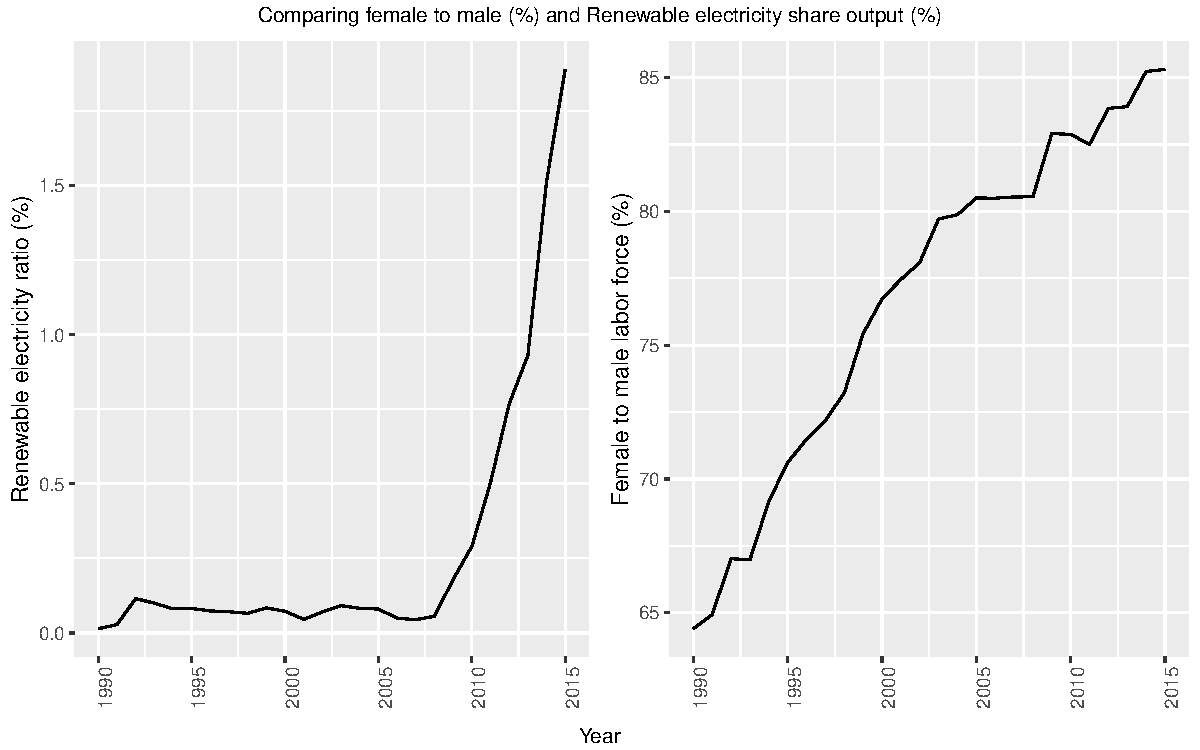
\includegraphics{report_files/figure-latex/compare-renewable-ftm-1.pdf}
\caption{\label{fig:compare-renewable-ftm}Comparing female to male ratio to renewable electricity output share}
\end{figure}

Comparing the ratio of female to male labor force participation rates to renewable electricity share in Figure \ref{fig:compare-renewable-ftm}, we note a more consistent growth of the ratio over time, whereas the renewable electricity ratio stays consistent until 2007, after which we observe a sharp increase. To understand this increase, we must delve more into the renewables future plan for Israel. Established in 2016 were steps to reach a target of 17\% Renewable Energy production by 2030, with interim targets of 10\% and 13\% by 2020/2023 respectively (\textcite{IEA2019}). Unfortunately, the data set used for this analysis does not have data past 2015, and as a result, we cannot identify the effect which the announcement could have made.

Looking at the change in electricity share in Figure \ref{fig:renewable-compare}:

\begin{figure}
\centering
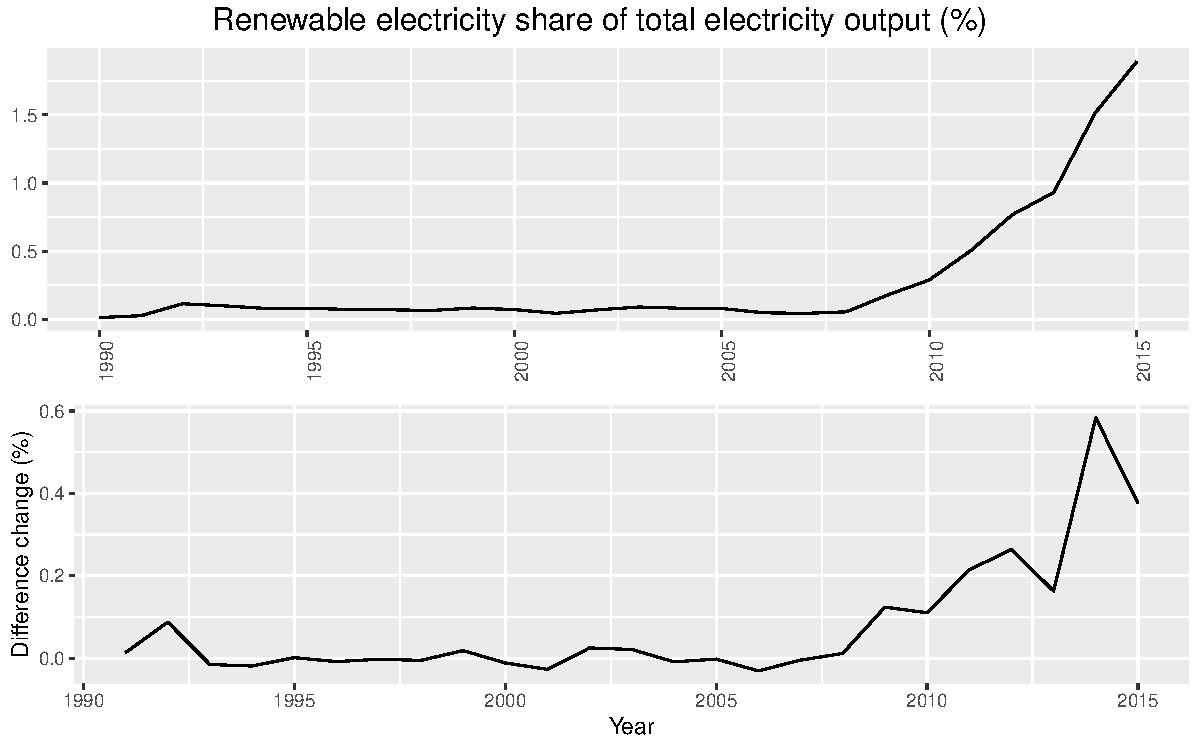
\includegraphics{report_files/figure-latex/renewable-compare-1.pdf}
\caption{\label{fig:renewable-compare}Looking at Renewable electricity share, and difference change}
\end{figure}

We can see that the difference seems to centre around zero prior to 2007, as was noted previously, however no clear perfect correlation can be seen when comparing the differences in Figure \ref{fig:renewable-compare} and Figure \ref{fig:compare-renewable-ftm}.

\pagebreak

\begin{table}[!h]

\caption{\label{tab:fcrenew}Forecast of renewable electricity share}
\centering
\fontsize{10}{12}\selectfont
\begin{tabular}[t]{lrr}
\toprule
  & Year & Renewable electricity share of total electricity output (\%)\\
\midrule
26 & 2016 & 1.965234\\
27 & 2017 & 2.040268\\
28 & 2018 & 2.115302\\
29 & 2019 & 2.190335\\
30 & 2020 & 2.265369\\
\bottomrule
\end{tabular}
\end{table}

Table \ref{tab:fcrenew} shows a forecast of the renewable electricity share of total electricity output in the next five years. This was conducted using a mean forecasting method. If current policies were followed, the target set in 2016 may not be met.

Perhaps, renewable energy is not exactly suitable in representing some change in attitude, Burke (\textcite{Burke2018}) and Sung (\textcite{Sung2018}) finds that renewable transition for the energy industry has been promoted by governments and markets, whereas traditional energy companies tend to hamper this progress. they also find that the general public do not have directly influence the transition, but indirectly affects it through the markets and governments. It may be suitable for the ratio of renewable energy output to proxy the strength of effect that the government/market has, and by extension, how the public affects decision making in the government.

Let's look at total energy consumed in relation to the female to male labour force ratio:

\begin{figure}
\centering
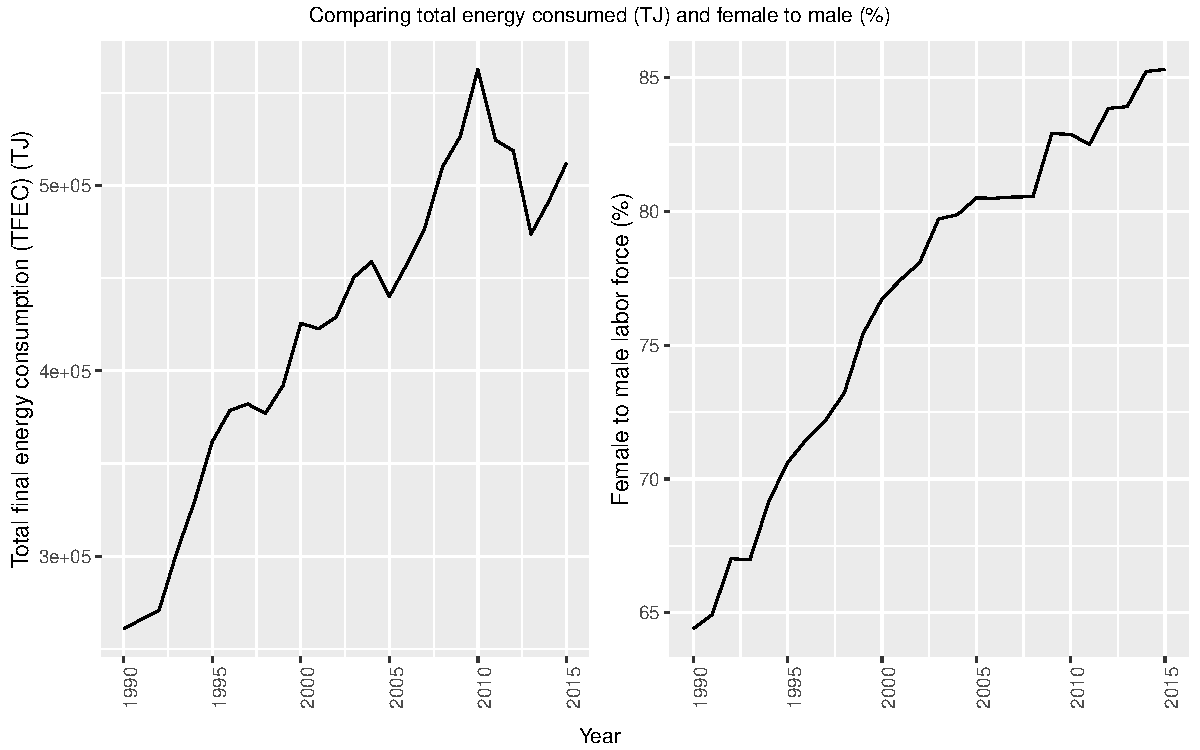
\includegraphics{report_files/figure-latex/energy-ftm-1.pdf}
\caption{\label{fig:energy-ftm}Comparing total energy consumption and female to male ratio.}
\end{figure}

We can see a similar trend between series in Figure \ref{fig:energy-ftm}. We could use total energy consumption as a way to proxy general changes in attitudes. Andrae (\textcite{Andrae2015}) discusses the general increase in electricity usage due to evolving communication technologies, including consumer devices. Here we note a significant increase in energy consumption over time, most likely attributable to an increased reliance on technology, including information technology. With a access to wider information, it is reasonable to expect some sort of changing attiude.

To conclude this section, we can use renewable electricity output ratio to directly model some government/market influence, and indirectly people. It may also be more reasonable to use total energy consumption to model changing attitudes.

\section*{Male and Female Mortality Rates and Birth Rate}

<<<<<<< HEAD
With Israel as our chosen country, this section will be analyzing the
relationship between our response variable, \emph{Ratio of female to
male labor force participation rate (\%) (national estimate)}, and the
following economic indicators: - Mortality rate, adult, female (per
1,000 female adults): Adult mortality rate, female, is the probability
of dying between the ages of 15 and 60--that is, the probability of a
15-year-old female dying before reaching age 60, if subject to
age-specific mortality rates of the specified year between those ages
(\textcite{TheWorldBank2018}) - Mortality rate, adult, male (per 1,000
male adults): Adult mortality rate, male, is the probability of dying
between the ages of 15 and 60--that is, the probability of a 15-year-old
male dying before reaching age 60, if subject to age-specific mortality
rates of the specified year between those ages
\textcite{TheWorldBank2018}). - Birth rate, crude (per 1,000 people):
Crude birth rate indicates the number of live births occurring during
the year, per 1,000 population estimated at midyear. Subtracting the
crude death rate from the crude birth rate provides the rate of natural
increase, which is equal to the rate of population change in the absence
of migration (\textcite{TheWorldBank2018}).

In order to assess their impact on the change of the female to male
labor force ratio to ultimately assess the potential change in how the
gender stereotype is percieved in Israel.

Across history, the traditional stereotype on gender roles has been one
that depicts males roles as the provider and women as the caretaker and
child bearer resulting in the notion that a woman's role is at home
which has led to less occupational opportunities and aspirations
\textcite{DickeAL2019}. These stereotypes are further perpetuated
through religion, as seen by the two most present religion in Israel -
Judaism and Islam where the traditional identity for involves leadership
for men and domesticity for females \textcite{Woodhead} in all facets of
life from work, private, public and in the army
(\textcite{GittlemenSI2020}). However, it does seem as though this
traditional view is being confronted and dismantled over time with more
religious and non religious Israeli woman taking up education and being
accepted in a range of occupational opportunities and army duties
\textcite{Levy2006}, as such birth rate and male and female mortality
rates are prime variables to potentially explain the change in the labor
force ratio thus indicating the potential change in how gender
stereotypes are viewed.

The variables for this section are isolated into their own data set in
both long and wide form.

\subsubsection{The variable change
overtime}\label{the-variable-change-overtime}
=======
With Israel as our chosen country, this section will be analyzing the relationship between our response variable, \emph{Ratio of female to male labor force participation rate (\%) (national estimate)}, and the following economic indicators:
- Mortality rate, adult, female (per 1,000 female adults): Adult mortality rate, female, is the probability of dying between the ages of 15 and 60--that is, the probability of a 15-year-old female dying before reaching age 60, if subject to age-specific mortality rates of the specified year between those ages (\textcite{TheWorldBank2018})
- Mortality rate, adult, male (per 1,000 male adults): Adult mortality rate, male, is the probability of dying between the ages of 15 and 60--that is, the probability of a 15-year-old male dying before reaching age 60, if subject to age-specific mortality rates of the specified year between those ages \textcite{TheWorldBank2018}).
- Birth rate, crude (per 1,000 people): Crude birth rate indicates the number of live births occurring during the year, per 1,000 population estimated at midyear. Subtracting the crude death rate from the crude birth rate provides the rate of natural increase, which is equal to the rate of population change in the absence of migration (\textcite{TheWorldBank2018}).

In order to assess their impact on the change of the female to male labor force ratio to ultimately assess the potential change in how the gender stereotype is percieved in Israel.

Across history, the traditional stereotype on gender roles has been one that depicts males roles as the provider and women as the caretaker and child bearer resulting in the notion that a woman's role is at home which has led to less occupational opportunities and aspirations \textcite{DickeAL2019}. These stereotypes are further perpetuated through religion, as seen by the two most present religion in Israel - Judaism and Islam where the traditional identity for involves leadership for men and domesticity for females \textcite{Woodhead} in all facets of life from work, private, public and in the army (\textcite{GittlemenSI2020}). However, it does seem as though this traditional view is being confronted and dismantled over time with more religious and non religious Israeli woman taking up education and being accepted in a range of occupational opportunities and army duties \textcite{Levy2006}, as such birth rate and male and female mortality rates are prime variables to potentially explain the change in the labor force ratio thus indicating the potential change in how gender stereotypes are viewed.

The variables for this section are isolated into their own data set in both long and wide form.

\hypertarget{the-variable-change-overtime}{%
\subsubsection{The variable change overtime}\label{the-variable-change-overtime}}
>>>>>>> 9024b81922d0500415b2610fbd1024857e6d728b

\begin{figure}
\centering
\includegraphics{report_files/figure-latex/combining-the-variable-figures-1.pdf}
\caption{\label{fig:combining-the-variable-figures}Each figure visualises the chosen variables}
\end{figure}

\begin{table}[!h]

\caption{\label{tab:percent-change-over-the-observed-time-period}The total percentage change from 1986 to 2016, per each variable}
\centering
\fontsize{7}{9}\selectfont
\begin{tabular}[t]{l|r|r|r}
\hline
Series & 1986 & 2016 & percent\_change\_1986\_to\_2016\\
\hline
Mortality rate, adult, male (per 1,000 male adults) & 130.69100 & 70.87300 & -45.770558\\
\hline
Mortality rate, adult, female (per 1,000 female adults) & 77.62700 & 39.63800 & -48.937870\\
\hline
Ratio of female to male labor force participation rate (\%) (national estimate) & 60.93083 & 85.91686 & 41.007207\\
\hline
Birth rate, crude (per 1,000 people) & 23.10000 & 21.20000 & -8.225108\\
\hline
\end{tabular}
\end{table}

<<<<<<< HEAD
Figure \ref{fig:combining-the-variable-figures} visualizes the change
over time for each of the chosen variables in this section, with the
selected variable on the y axis and year along the x axis.

Key takeaways: - The labor force participation figure shows that the
ratio of female to male labor force participation rate has increased
from 1986 to 2016, by 41.01\% as shown by Table
\ref{tab:percent-change-over-the-observed-time-period}. - The birth rate
figure shows the birth rate per 1000 people overall shows a reduction in
the birth rate has increased from 1986 to 2016, by -8.23\% as shown by
Table \ref{tab:percent-change-over-the-observed-time-period}. - The
mortality rate table shows the mortality rate for females per 1000
female adults in orange and the mortality rate for males per 1000 males
in blue. Both indicators have reduced from 1986 to 2016 at a relatively
even rate, with female mortality reducing by -48.94\% and male mortality
reducing by -45.80\%, as shown by Table
\ref{tab:percent-change-over-the-observed-time-period}.

\subsubsection{Correlation comparison}\label{correlation-comparison}

The explanatory variables are presented as ratios and in order for their
results to be relative to the explanatory variable and to allow for
analysis to take place, they are turned into percentages. The new column
percent\_value shows the percentage of birth rate and female and male
mortality rates for every 1000 people, from which a new data set will be
created showing the percentage results for all the variables in this
section.
=======
Figure \ref{fig:combining-the-variable-figures} visualizes the change over time for each of the chosen variables in this section, with the selected variable on the y axis and year along the x axis.

Key takeaways:
- The labor force participation figure shows that the ratio of female to male labor force participation rate has increased from 1986 to 2016, by 41.01\% as shown by Table @ref(tab:pct\_change\_mortality\_variables).
- The birth rate figure shows the birth rate per 1000 people overall shows a reduction in the birth rate has increased from 1986 to 2016, by -8.23\% as shown by Table @ref(tab:pct\_change\_mortality\_variables).
- The mortality rate table shows the mortality rate for females per 1000 female adults in orange and the mortality rate for males per 1000 males in blue. Both indicators have reduced from 1986 to 2016 at a relatively even rate, with female mortality reducing by -48.94\% and male mortality reducing by -45.80\%, as shown by Table @ref(tab:pct\_change\_mortality\_variables).

\hypertarget{correlation-comparison}{%
\subsubsection{Correlation comparison}\label{correlation-comparison}}

The explanatory variables are presented as ratios and in order for their results to be relative to the explanatory variable and to allow for analysis to take place, they are turned into percentages. The new column percent\_value shows the percentage of birth rate and female and male mortality rates for every 1000 people, from which a new data set will be created showing the percentage results for all the variables in this section.
>>>>>>> 9024b81922d0500415b2610fbd1024857e6d728b

\textbackslash{}begin\{table\}{[}!h{]}

\textbackslash{}caption\{\label{tab:correlation-between-response-explanatory}The correlation between the percentage results, per 1000 people, of the response variables and the ratio of female to male labor force participation rate (\%)\}
\centering

\begin{tabular}[t]{r|r|r}
\hline
correlation\_results\_male\_mort & correlation\_results\_female\_mort & correlation\_results\_birth\_rate\\
\hline
-0.9602867 & -0.9889846 & -0.6043269\\
\hline
\end{tabular}

\textbackslash{}end\{table\}

\begin{figure}
\centering
\includegraphics{report_files/figure-latex/figure-correlation-female-mort-labor-force-1.pdf}
\caption{\label{fig:figure-correlation-female-mort-labor-force}The figure displays the relationship between the percentage results of female mortality rates per 1000 adult females and the Ratio of female to male labor force participation rate (\%) (national estimate)}
\end{figure}

\begin{figure}
\centering
\includegraphics{report_files/figure-latex/figure-correlation-male-mort-labor-force-1.pdf}
\caption{\label{fig:figure-correlation-male-mort-labor-force}The figure displays the relationship between the percentage results of male mortality rates per 1000 adult females and the Ratio of female to male labor force participation rate (\%) (national estimate)}
\end{figure}

\begin{figure}
\centering
\includegraphics{report_files/figure-latex/figure-correlation-birth-rate-labor-force-1.pdf}
\caption{\label{fig:figure-correlation-birth-rate-labor-force}The figure displays the relationship between the percentage results of birth rates per 1000 adult females and the Ratio of female to male labor force participation rate (\%) (national estimate)}
\end{figure}

<<<<<<< HEAD
Figure \ref{fig:figure-correlation-birth-rate-labor-force} visualizes
the correlation between birth rate and the female to male labor force
ratio, with birth rate, crude (per 1,000 people) on the y axis and the
ratio of female to male labor force participation rate on the x axis.
The figure shows a negative correlation between the two variables
however, there are some scattered results where both birth rate and
female to male labor force ratio are both relatively low which is
depicted by the correlation coefficient of -0.60 as shown by Table
\ref{tab:correlation-between-response-explanatory}.

Figure \ref{fig:figure-correlation-male-mort-labor-force} visualizes the
correlation between male mortality rate and the female to male labor
force ratio, with male mortality rate per 1,000 male adults on the y
axis and the ratio of female to male labor force participation rate on
the x axis. The figure displays a strong negative correlation between
the two variables which is backed up by the correlation coefficient of
-.96 in Table \ref{tab:correlation-between-response-explanatory}.

Figure \ref{fig:figure-correlation-female-mort-labor-force} visualizes
the correlation between female mortality rate and the female to male
labor force ratio, with female mortality rate per 1,000 female adults on
the y axis and the ratio of female to male labor force participation
rate on the x axis. The figure displays a strong negative correlation
between the two variables which is backed up by the correlation
coefficient of -.99 in Table
\ref{tab:correlation-between-response-explanatory}.

As evident by the analysis conducted in this section, there is a clear
positive correlation between the three explanatory variables and the the
ratio of female to male labor force participation rate. However, the
causality and the significance of the relationship between the
explanatory variables and the response variable is yet to be determined
so despite seeing a consistent correlation between the variables,
further analysis is required to determine how significant the
relationship is.
=======
Figure \ref{fig:figure-correlation-birth-rate-labor-force} visualizes the correlation between birth rate and the female to male labor force ratio, with birth rate, crude (per 1,000 people) on the y axis and the ratio of female to male labor force participation rate on the x axis. The figure shows a negative correlation between the two variables however, there are some scattered results where both birth rate and female to male labor force ratio are both relatively low which is depicted by the correlation coefficient of -0.60 as shown by Table \ref{tab:correlation-between-response-explanatory}.

Figure \ref{fig:figure-correlation-male-mort-labor-force} visualizes the correlation between male mortality rate and the female to male labor force ratio, with male mortality rate per 1,000 male adults on the y axis and the ratio of female to male labor force participation rate on the x axis. The figure displays a strong negative correlation between the two variables which is backed up by the correlation coefficient of -.96 in Table \ref{tab:correlation-between-response-explanatory}.

Figure \ref{fig:figure-correlation-female-mort-labor-force} visualizes the correlation between female mortality rate and the female to male labor force ratio, with female mortality rate per 1,000 female adults on the y axis and the ratio of female to male labor force participation rate on the x axis. The figure displays a strong negative correlation between the two variables which is backed up by the correlation coefficient of -.99 in Table \ref{tab:correlation-between-response-explanatory}.

As evident by the analysis conducted in this section, there is a clear positive correlation between the three explanatory variables and the the ratio of female to male labor force participation rate. However, the causality and the significance of the relationship between the explanatory variables and the response variable is yet to be determined so despite seeing a consistent correlation between the variables, further analysis is required to determine how significant the relationship is.
>>>>>>> 9024b81922d0500415b2610fbd1024857e6d728b

\section*{Labour Force Analysis}

\hypertarget{overview}{%
\section{Overview}\label{overview}}

This section of the report will focus on analysing various aspects of the Israeli labour force with respect to the research question that we have chosen which is ``How have the views towards gender stereotypes changed over time in Israel?''. The Israeli labour force has come a long way from being male dominated to being almost equally divided between men and women. The transition of the Israeli labour force shall be explored through the years 1991-2019 in this section of the report.

\begin{table}[!h]

\caption{\label{tab:showcase}Variables Summary}
\centering
\begin{tabular}[t]{>{\raggedright\arraybackslash}p{2em}|>{\raggedleft\arraybackslash}p{5em}|>{\raggedleft\arraybackslash}p{5em}|>{\raggedleft\arraybackslash}p{5em}|>{\raggedleft\arraybackslash}p{5em}|>{\raggedleft\arraybackslash}p{5em}|>{\raggedleft\arraybackslash}p{5em}}
\hline
Year & Labor force, female (\% of total labor force) & Ratio of female to male labor force participation rate (\%) (national estimate) & Self-employed, female (\% of female employment) (modeled ILO estimate) & Wage and salaried workers, female (\% of female employment) (modeled ILO estimate) & Labor force participation rate, male (\% of male population ages 15-64) (modeled ILO estimate) & Labor force participation rate, female (\% of female population ages 15-64) (modeled ILO estimate)\\
\hline
1991 & 40.15476 & 64.92514 & 5.907 & 94.093 & 78.995 & 53.404\\
\hline
1992 & 41.07230 & 67.01756 & 5.932 & 94.068 & 78.643 & 55.041\\
\hline
1993 & 41.16972 & 66.97746 & 5.900 & 94.100 & 80.463 & 56.408\\
\hline
1994 & 42.01045 & 69.15992 & 5.895 & 94.105 & 80.645 & 58.274\\
\hline
1995 & 42.60488 & 70.61269 & 5.909 & 94.091 & 80.267 & 59.313\\
\hline
1996 & 43.00450 & 71.47999 & 6.159 & 93.841 & 79.046 & 59.308\\
\hline
\end{tabular}
\end{table}

Table \ref{tab:showcase} exhibits the variables that have been used in this section of the report and displays the first 5 rows. The ratio of self-employed females is the explanatory variable and the ratio of female to male participation rate is the response variable.The table gives a brief overview of how the variables change from the period 1991-1996.

\begin{figure}
\centering
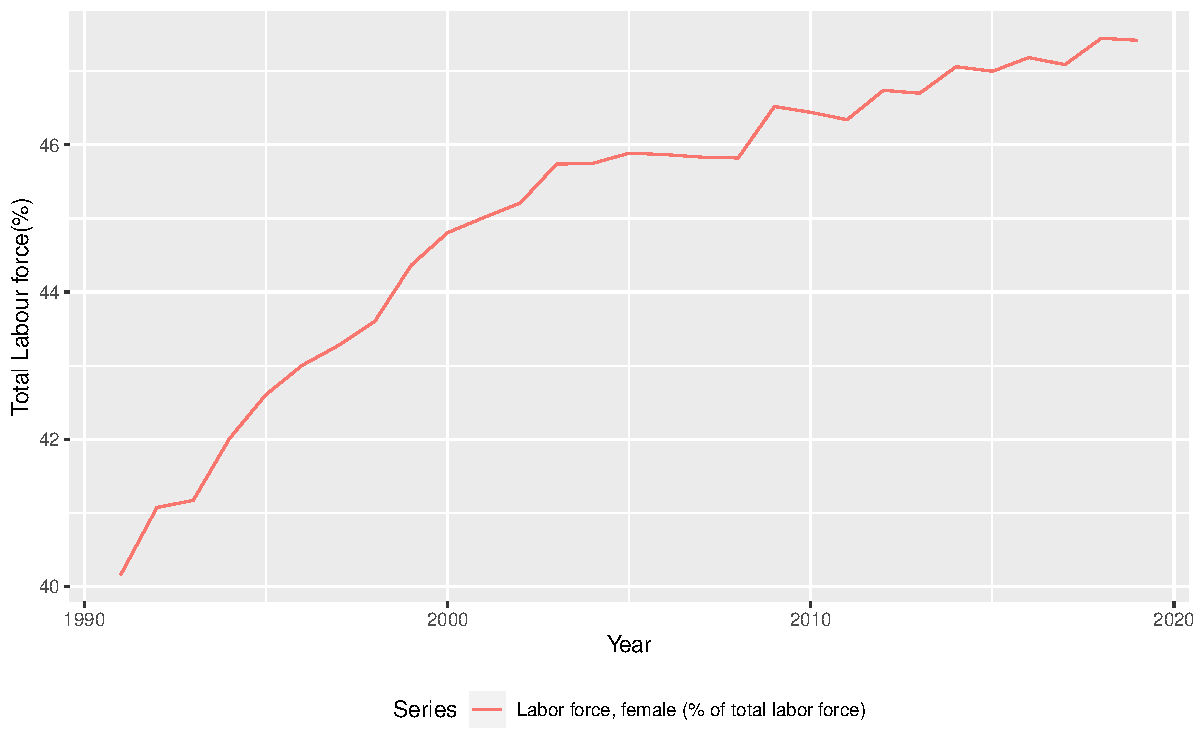
\includegraphics{report_files/figure-latex/graph1-1.pdf}
\caption{\label{fig:graph1}\% Female labour force out of total labour force}
\end{figure}

Figure \ref{fig:graph1} depicts the gentle rise in the female labour force which was around 40\% of the total labour force in 1990 to around 47\% around 2020. One of the main reasons behind the surge in female participation is due to the educational attainment of women in Israel. Also, in 2006 and 2007 numerous amendments were made to women employment law to protect the rights of women at workplace and provide equal employment opportunities which has proved to be pivotal in increasing female participation in the labour force \autocite{israelministryofforeignaffairs2013}.

\hypertarget{self-employed-vs-wage-salaried-women}{%
\section{Self-employed v/s wage \& salaried women}\label{self-employed-vs-wage-salaried-women}}

\begin{figure}
\centering
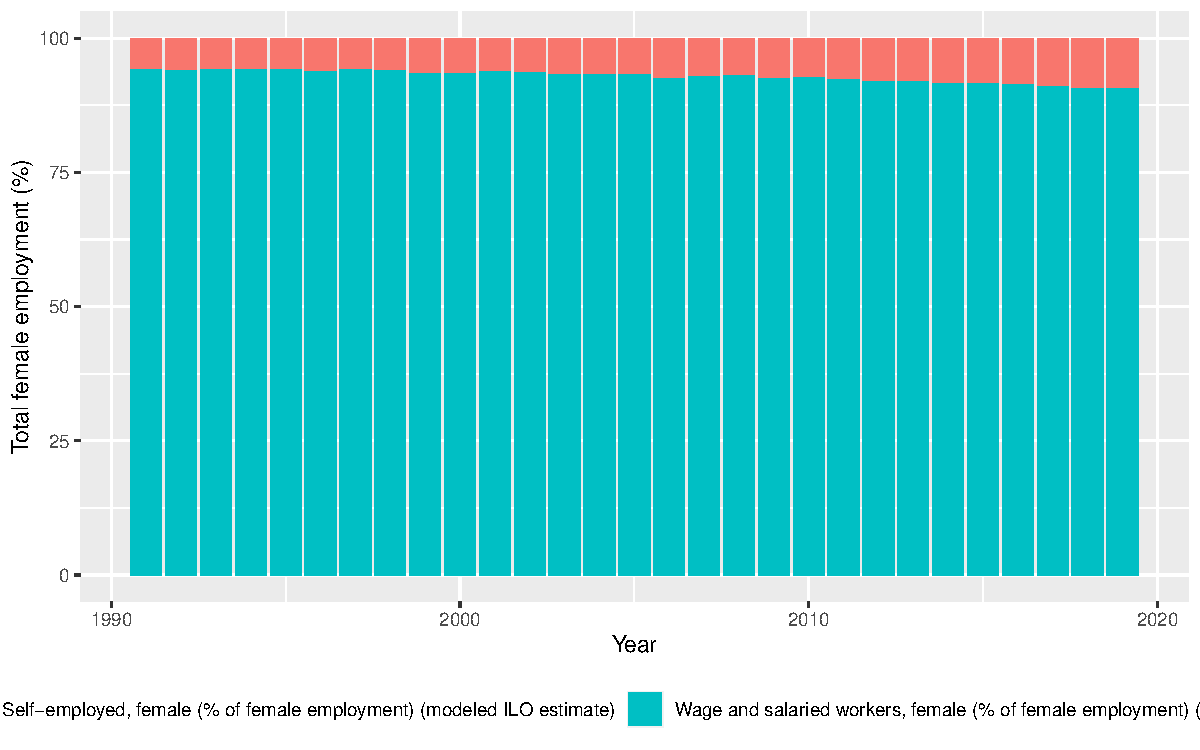
\includegraphics{report_files/figure-latex/graph2-1.pdf}
\caption{\label{fig:graph2}Self-employed v/s Wage \& salaried female workers}
\end{figure}

Figure \ref{fig:graph2} shows the slow but gradual increase in the percentage of self-employed females in the female labour workforce. The female labour workforce comprises of self-employed women and wage and salaried women. The percentage of self-employed women in Israel has increased from 5.9 to 9.2 in 3 decades. The gradual change can be attributed to strong family orientation present in the Israeli culture and the fact that a working mother has to always give priorities to family responsibilities. But the main contributing factor to the increase was achievement motivations and economic necessities more than educational attainment or previous entrepreneurial experience. \textcite{lerner1997israeli}

\hypertarget{female-vs-male-labour-force-participation}{%
\section{Female v/s Male labour force participation}\label{female-vs-male-labour-force-participation}}

\begin{figure}
\centering
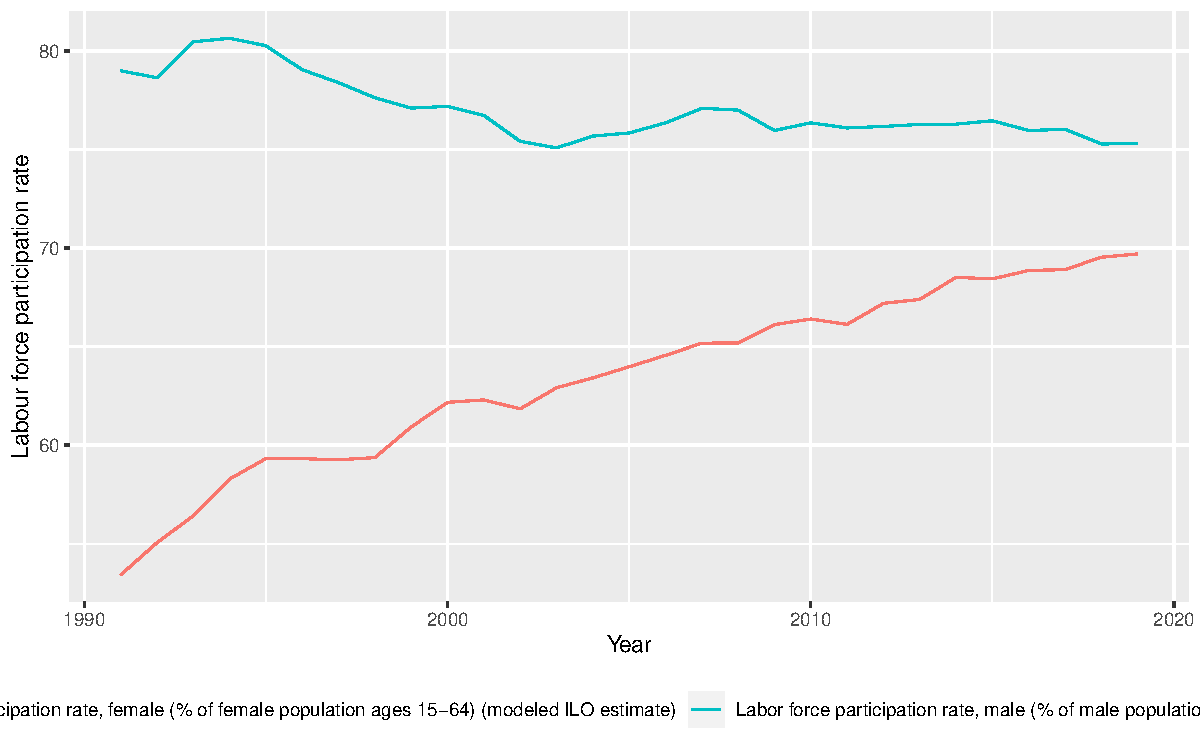
\includegraphics{report_files/figure-latex/graph3-1.pdf}
\caption{\label{fig:graph3}Female v/s Male labour force participation}
\end{figure}

Figure \ref{fig:graph3} compares the female v/s male labour force participation amongst the total population in the age group of 15-64 females and males respectively. It depicts the percentage of the female population that is engaged in the labour force in the working age population. This is a very good representation of the increased number of participation of women in the labour force which has increased almost 20\% in the past 30 years which authenticates that views towards gender stereotypes are changing over time in Israel. This shows that Israeli women are more willing and motivated to be involved in the labour force than they ever were.

\hypertarget{female-labour-force-vs-female-male-participation-rate}{%
\section{Female labour force v/s female-male participation rate}\label{female-labour-force-vs-female-male-participation-rate}}

\begin{figure}
\centering
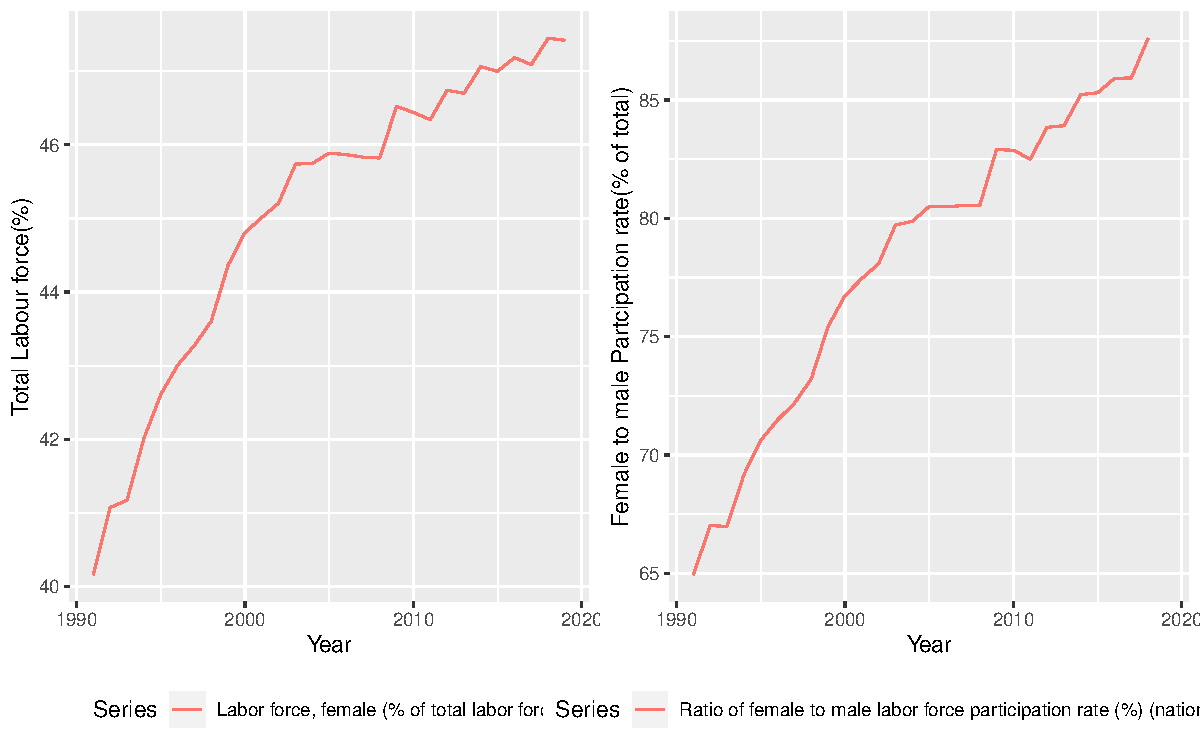
\includegraphics{report_files/figure-latex/graph5-1.pdf}
\caption{\label{fig:graph5}Comparing female labour force with female-male participation rate}
\end{figure}

Figure \ref{fig:graph5} verifies that the percentage of females in the total labour force is positively correlated with the female to male labour force participation rate as both show a positive trend over time and have increased significantly since 1991 to 2019.

\section*{Model}

<<<<<<< HEAD
A linear regression model was developed to explore the impact of the
variables we have researched in the previous sections on our target
variable
\texttt{Ratio\ of\ female\ to\ male\ labor\ force\ participation\ rate\ (\%)\ (national\ estimate)}.
The variables chosen were:

\begin{itemize}
\tightlist
\item
  Birth rate, crude (per 1,000 people)
\item
  Self-employed, female (\% of female employment) (modeled ILO estimate)
\item
  Adjusted savings: education expenditure (current US\$)
\item
  Total final energy consumption (TFEC) (TJ)
\end{itemize}

To match the series, and avoid imputing missing values, we have selected
a time range between 1991 and 2015 to conduct our regression.
=======
A linear regression model was developed to explore the impact of the variables we have researched in the previous sections on our target variable \texttt{Ratio\ of\ female\ to\ male\ labor\ force\ participation\ rate\ (\%)\ (national\ estimate)}. The variables chosen were:
\textbackslash{}begin\{itemize\}

\item

Birth rate, crude (per 1,000 people)

\item

Self-employed, female (\% of female employment) (modeled ILO estimate)

\item

Adjusted savings: education expenditure (current US\$)

\item

Total final energy consumption (TFEC) (TJ)
\textbackslash{}end\{itemize\}

To match the series, and avoid imputing missing values, we have selected a time range between 1991 and 2015 to conduct our regression.
>>>>>>> 9024b81922d0500415b2610fbd1024857e6d728b

A summary of the model has detailed in Table \ref{tab:model-summary}

\begin{table}[!h]

\caption{\label{tab:model-summary}Linear regression summary}
\centering
<<<<<<< HEAD
\fontsize{7}{9}\selectfont
=======
\fontsize{10}{12}\selectfont
>>>>>>> 9024b81922d0500415b2610fbd1024857e6d728b
\begin{tabular}[t]{lrrrr}
\toprule
term & estimate & std.error & statistic & p.value\\
\midrule
(Intercept) & 69.5100838 & 26.0317844 & 2.6702005 & 0.0147048\\
`Birth rate, crude (per 1,000 people)` & -1.6026066 & 1.1670520 & -1.3732092 & 0.1848878\\
`Adjusted savings: education expenditure (current US\$)` & 0.0000000 & 0.0000000 & -0.5971594 & 0.5571017\\
`Self-employed, female (\% of female employment) (modeled ILO estimate)` & 3.0222842 & 1.0603237 & 2.8503412 & 0.0098895\\
`Total final energy consumption (TFEC) (TJ)` & 0.0000529 & 0.0000066 & 8.0435848 & 0.0000001\\
\bottomrule
\end{tabular}
\end{table}

<<<<<<< HEAD
From this result, we find that
\texttt{Total\ final\ energy\ consumption\ (TFEC)\ (TJ)} is
statistically significant at all levels. One possible reason is the
relationship between electricity usage and changing attitudes. As
previously discussed, one cause of greater energy usage is the
increasing use of communications and information technology. With wider
access to a different range of opinions, newer generations are less
likely to share the same values with previous generation, hence
justifying the change in attitude.

Interestingly noted is the weaker signficance of the variable
\texttt{Self-employed,\ female\ (\%\ of\ female\ employment)\ (modeled\ ILO\ estimate)}.
As noted previously, there is a strong correlation between this and the
target variable. One reason this may be the case is that family
orientation is emphasised in Israeli culure. Working mothers prioritise
family repsonsibilities hence are less inclined to self-employ
themselves.

\section*{Conclusion}

To conclude our report, we can observe the gender stereotype lessening
to some degree. The individual variables which we have selected can
explain why this is the case to a certain degree, however to obtain
meaningful results, further research must be conducted. It is also
important to note that only recently has gender equality been an issue
so widely recognised. More data may be required to explore how different
variables interact with equality in today's world.

References
=======
From this result, we find that \texttt{Total\ final\ energy\ consumption\ (TFEC)\ (TJ)} is statistically significant at all levels. One possible reason is the relationship between electricity usage and changing attitudes. As previously discussed, one cause of greater energy usage is the increasing use of communications and information technology. With wider access to a different range of opinions, newer generations are less likely to share the same values with previous generation, hence justifying the change in attitude.

Interestingly noted is the weaker signficance of the variable \texttt{Self-employed,\ female\ (\%\ of\ female\ employment)\ (modeled\ ILO\ estimate)}. As noted previously, there is a strong correlation between this and the target variable. One reason this may be the case is that family orientation is emphasised in Israeli culure. Working mothers prioritise family repsonsibilities hence are less inclined to self-employ themselves.

\section*{Conclusion}

To conclude our report, we can observe the gender stereotype lessening to some degree. The individual variables which we have selected can explain why this is the case to a certain degree, however to obtain meaningful results, further research must be conducted. It is also important to note that only recently has gender equality been an issue so widely recognised. More data may be required to explore how different variables interact with equality in today's world.

\pagebreak
>>>>>>> 9024b81922d0500415b2610fbd1024857e6d728b

\printbibliography

\end{document}

